\chapter{Dise\~no del sistema de distribución de carga}
\label{cap:disenoSistema}

Como se hizo mención en el Capítulo \ref{cap:introduccion}, el problema de la sobrecarga en un SPS está dado por el carácter estático del diseño de la aplicación, una vez comenzado la ejecución de ésta. Esto quiere decir, que en el momento que el sistema está en ejecución, no existen un mecanismo que permita adaptar los recursos a las necesidades actuales del sistema, por lo que se vuelve ineficiente, pudiendo generar sobrecargas en los operadores que lo componen.

Bajo un escenario como este, es necesario un sistema dinámico, que pueda adaptar su estructura, dependiendo de la carga y el flujo de datos recibidos. Considerando esta problemática, se diseñó un sistema que se adapta de manera automática a las condiciones de tráfico y carga, logrando optimizar su rendimiento, sin comprometer de manera significativa el \textit{performance} del sistema.

\section{Análisis del sistema de distribución de carga}
Dentro del análisis realizado en la arquitectura del sistema implementando, se consideró una perspectiva en base a los recursos lógicos según el enfoque dinámico, definido en las subsección \ref{subsec:recLogicosBC} y \ref{subsec:enfoqueDinamicoBC} respectivamente, para el balance de carga de SPS. El presente trabajo no se enfoca en el análisis del comportamiento de cada uno de los nodos físicos del sistema, sino que más bien en el estado de cada uno de los operadores del grafo diseñado, siendo un problema de carácter lógico y no físico.

Respecto al estudio de las distintas técnicas implementadas, era necesario utilizar una que no perdiera o minimizara la pérdida de datos, que fuera capaz de adaptarse a las condiciones dinámicas del tráfico, y que introdujera un bajo \textit{overhead} al sistema, de tal manera que sea escalable. Bajo estas restricciones, se consideró que la mejor opción era utilizar la técnica de fisión, utilizando el mismo modelo de replicación que Fernández \citep{FernandezMKP13}, donde basándose en el nivel de carga del operador se genera o no una réplica para este. Dentro de las hipótesis planteadas, se pensaba que el costo de un operador iba a ser menor a la formación de las colas de datos en el sistema, lo cual podría variar según la arquitectura del SPS implementando.

En la Figura \ref{fig:ejReplicacion} se muestra un ejemplo de la replicación propuesta, donde en la Subfigura (a) se presentan tres operadores, en uno de ellos (operador B) existe una sobrecarga, por lo que es necesario replicar el operador. En la Subfigura (b) se presenta el operador ya replicado, pero todavía persiste la sobrecarga en éste, por lo que se vuelve a realizar el mismo procedimiento, hasta que finalmente converge a la cantidad óptima de réplicas deseadas en el sistema en el período de tiempo analizado, como se muestra en la Subfigura (c).

\begin{figure}[!hb]
	\centering
		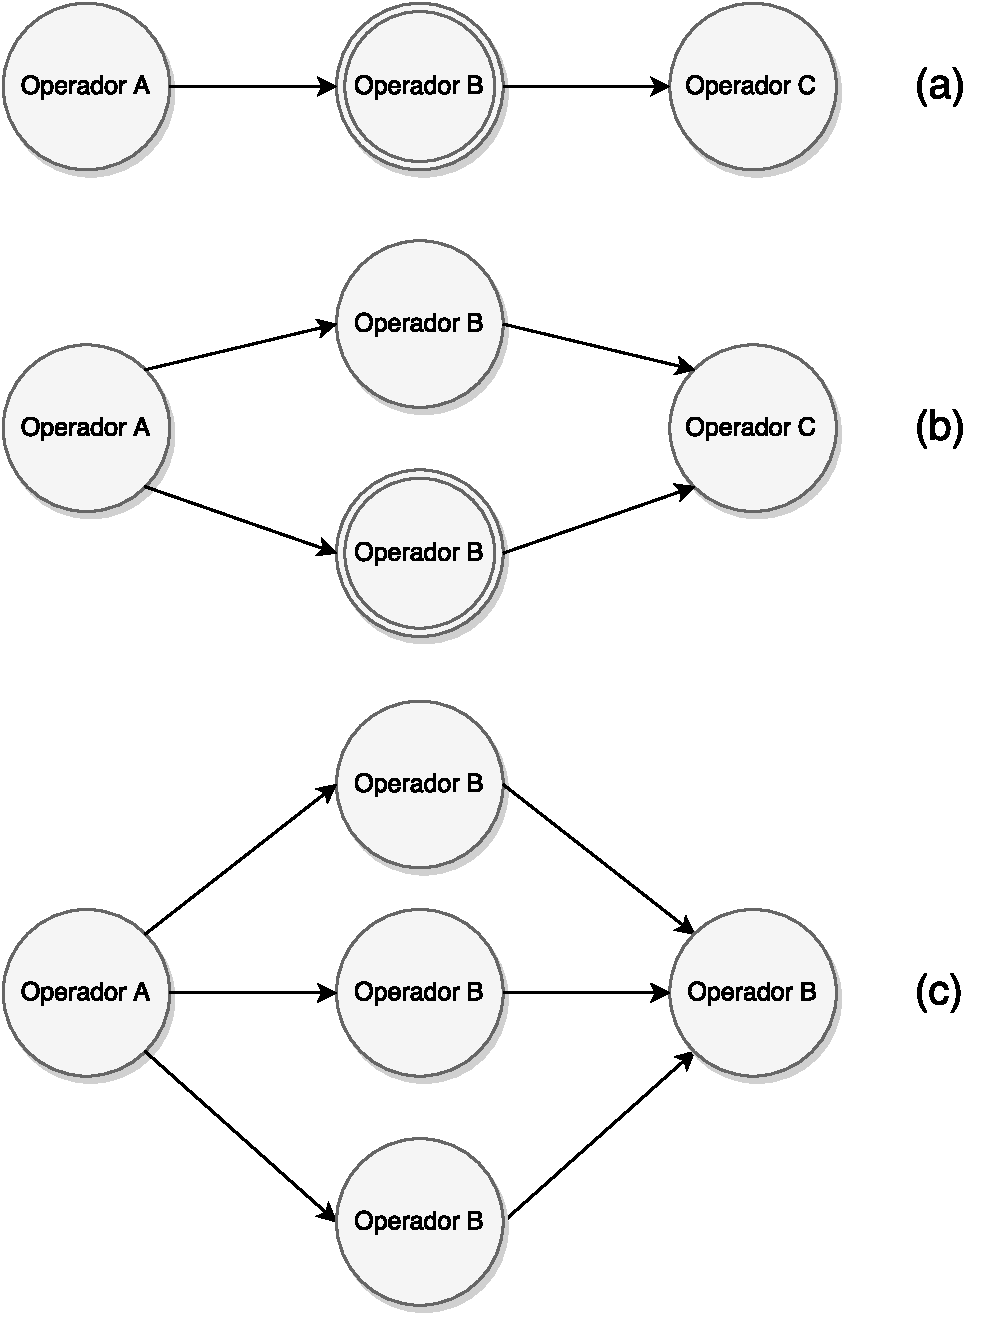
\includegraphics[scale=0.6]{images/EjReplicacion.pdf}
	\caption{Ejemplo de replicación del sistema propuesto.}
	\label{fig:ejReplicacion}
\end{figure}

%Para el diseño del sistema, era necesario contar con un umbral que determinara cuando el operador está o no sobrecargado, por lo que para esto se utilizaron conceptos de teoría de colas \citep{bose2013introduction}. Como los SPS están orientados en grafos, se posee tanto la tasa de llegada ($\lambda$) como la tasa de procesamiento ($\mu$) para cada uno de los operadores, como se ve representando en la Figura \ref{fig:analisisTeoriaColas}, donde la tasa de procesamiento de un operador es la misma tasa de llegada del siguiente operador en el grafo. Utilizando este tipo de conceptos, para cada operador se calculó la tasa de procesamiento ($\rho$), la cual esta definida por la tasa de llegada, la tasa de procesamiento y la cantidad de servicios disponibles en el sistema ($\rho = \frac{\lambda}{\mu \rho}$), cuyo valor nos indica el rendimiento del operador en cierta período de tiempo.

Para la detección del nivel de carga de un operador es necesario contar con un modelo basado en umbrales que permitan determinar cuando está o no sobrecargado un operador. Para modelar esta situación se utilizaron conceptos de teoría de colas \citep{bose2013introduction}. Dado que los SPS se encuentran en el paradigma orientado a grafos, se puede obtener tanto la tasa de llegada ($\lambda$) como la tasa de servicio ($\mu$) de cada uno de los operadores que lo componen, como se ve representando en la Figura \ref{fig:analisisTeoriaColas}. Aquí la tasa de procesamiento de un operador influye directamente en la tasa de llegada del siguiente operador en el grafo. Al utilizar estos conceptos, se cálculo la tasa de rendimiento ($\rho$), la cual está definida por la tasa de llegada, de procesamiento y la cantidad de réplicas del operador ($\rho = \frac{\lambda}{\mu \rho}$), cuyo valor representa el factor de utilización del sistema, donde se define un sistema estable si y sólo si $\rho < 1$.

\begin{figure}[!hb]
	\centering
		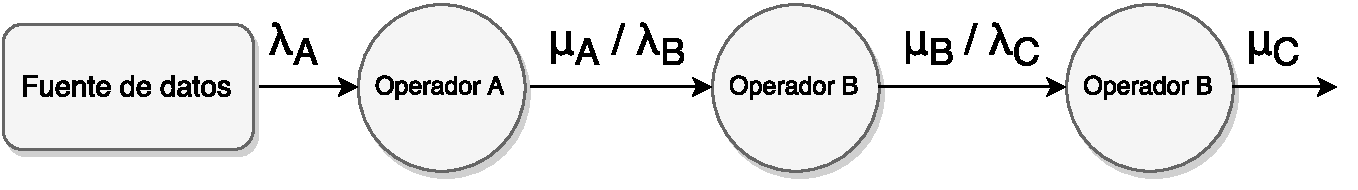
\includegraphics[scale=0.6]{images/AnalisisTeoriaColas.pdf}
	\caption{Enfoque de un SPS con conceptos de teoría de colas.}
	\label{fig:analisisTeoriaColas}
\end{figure}

Tomando en consideración el tipo de enfoque en el algoritmo de balance de carga y la elasticidad que se pretendía por parte del sistema, es que se trataron tres posibles estados en el sistema: ocioso, estable e inestable. El primer estado corresponde a un exceso en la cantidad de recursos asignados. El segundo está definido por el rendimiento óptimo del sistema. Y por último, el tercero hace referencia a un sistema sobrecargado, donde es necesario una mayor cantidad de recursos por parte de éste. Definido los posibles estados de cada operador, es que se tomó esto como base para el análisis y predicción de la carga en el sistema de distribución de carga.

Para el sistema propuesto, se consideraron dos tipos de algoritmos: predictivo, enfocado en el futuro y la historia del operador, y reactivo, analizando el comportamiento del momento. Esto fue diseñado con el fin de analizar dos factores, los \textit{peak} existentes en la historia del operador, dado el algoritmo predictivo, y otro que analice el comportamiento en el momento, haciendo uso del algoritmo reactivo, de tal manera de solucionar los comportamientos que no son detectados con la predicción.

Es importante denotar que dependiendo del tipo de caso es que un tipo de algoritmos va a funcionar mejor. Por ejemplo, si existe una variación muy alta en una período de tiempo considerable, el algoritmo predictivo puede detectar este tipo de \textit{peaks}. De esta manera, la predicción es más asertiva que el análisis en el momento. Pero en casos que no exista este tipo de casos, y sólo hayan variaciones en ciertos instantes de la ejecución, se encuentra el algoritmo reactivo para analizar el estado del operador.

Además de lo anterior, se consideró que era necesario trabajar con los dos algoritmos en temporalidades distintas, es decir, en cierto período de tiempo se va a utilizar el reactivo y en otro el predictivo. Esto quiere decir que mientras se obtienen las $n$ muestras para realizar el cálculo de predictivo, el algoritmo reactivo está realizando un análisis de los distintos operadores.

%Al diseñar un sistema que pudiera lidiar con dos tipos de algoritmos, era necesario considerar un algoritmo que pudiera administrar la cantidad de cargas, con tal utilizar el algoritmo necesario según el período existente en una ventana de tiempo, como también la cantidad de réplicas que deben aplicarse.

Como se diseñaron dos tipos de algoritmos que se complementan, es necesario considerar un algoritmo que administre cual de los dos algoritmos se va a utilizar según el período analizado, como también la cantidad de réplicas que deben crearse o eliminar según el resultado del algoritmo utilizado.

Dado lo anterior, se diseño un sistema elástico de distribución de carga con cuatro componentes: monitor de carga, analizador de carga, predictor de carga y administrador de réplicas, que se pueden apreciar en la Figura \ref{fig:componentesSistemas}.

\begin{figure}[ht!]
  \centering
    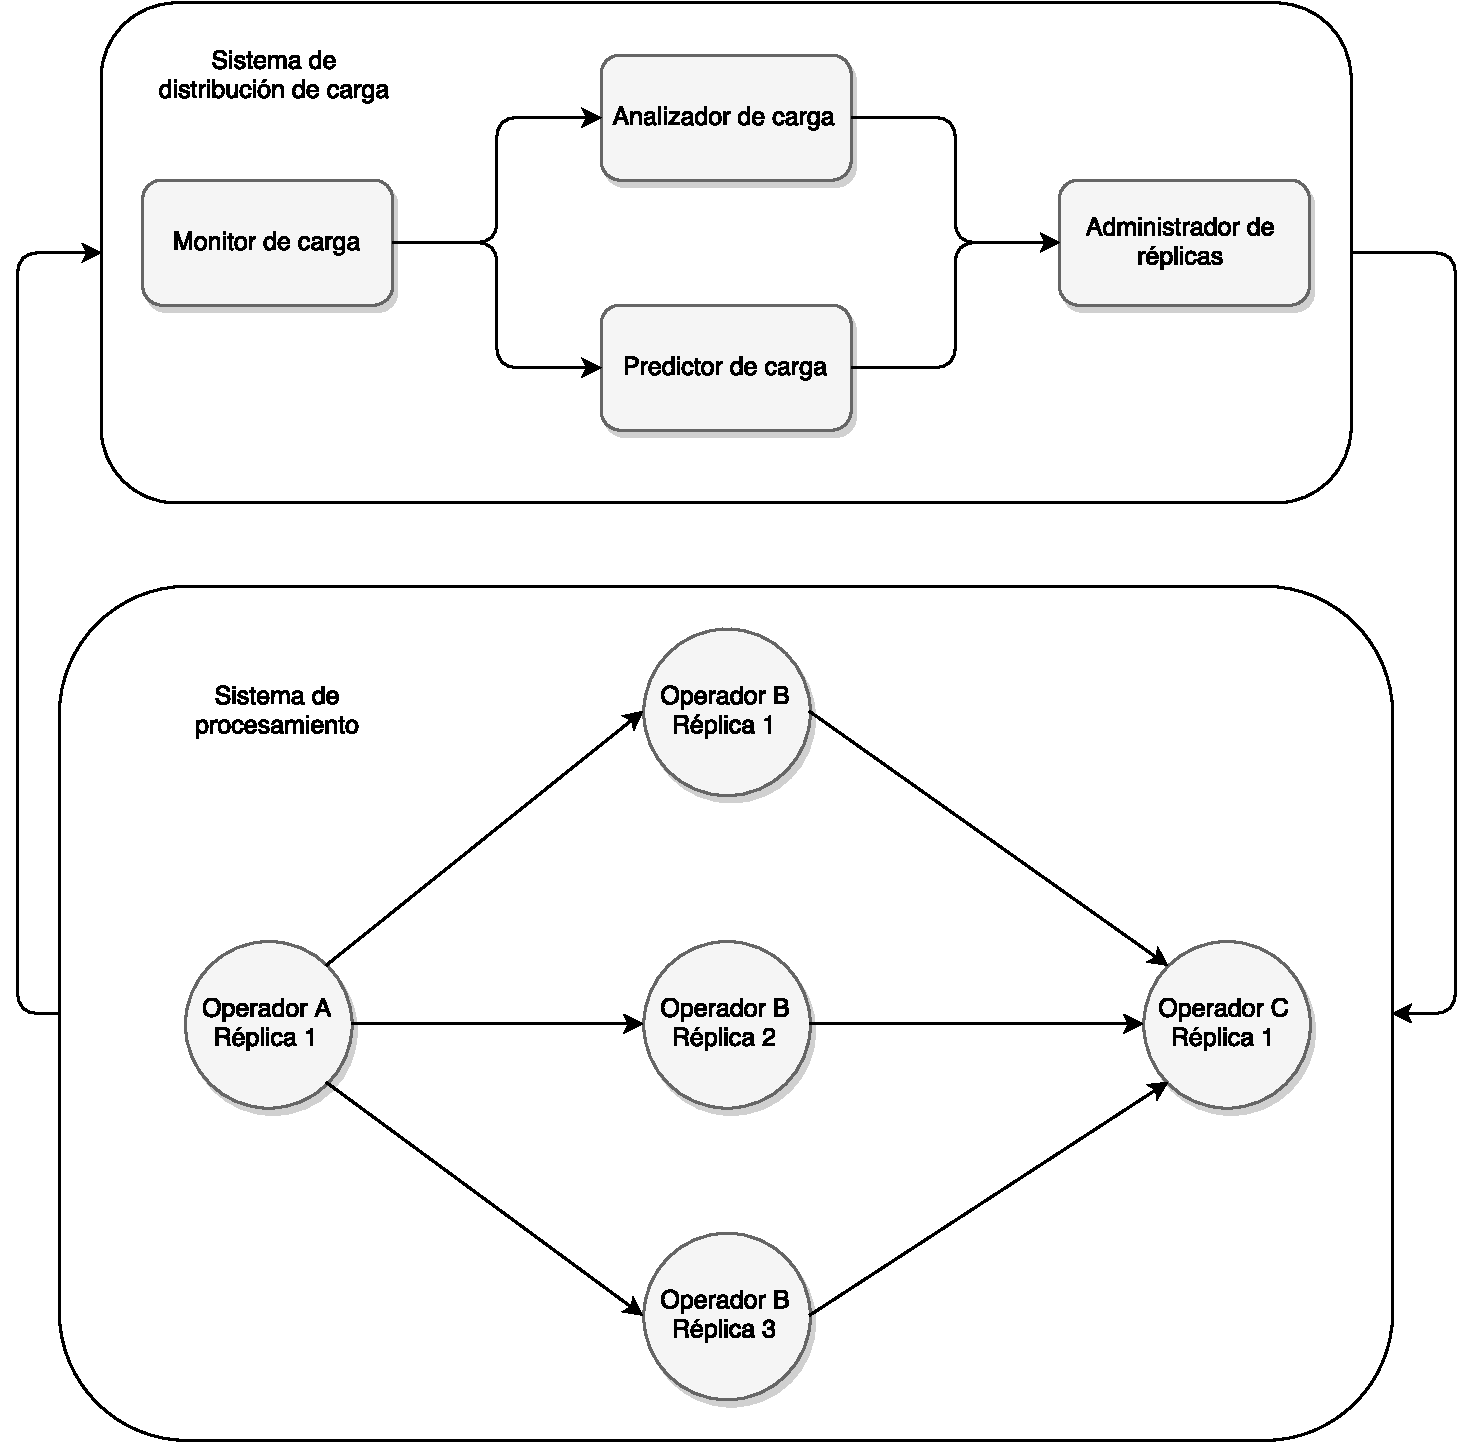
\includegraphics[scale=0.5]{images/Diagrama.pdf}
  \caption{Estructura del sistema de distribución de carga.}
  \label{fig:componentesSistemas}
\end{figure}

\paragraph{Monitor de carga:} está encargado de recolectar las estadísticas del sistema, tanto para el algoritmo reactivo, como para el historial del algoritmo predictivo.

\paragraph{Analizador de carga:} analiza la cantidad de carga de un operador en un período de tiempo determinado según el algoritmo reactivo, y respecto a esto se indica el estado del operador. Para esto, se consideró la tasa de rendimiento del operador, y según el valor que posea se determinará el estado, el cual podía ser ocioso, estable o inestable.

\paragraph{Predictor de carga:} es el módulo del algoritmo predictivo, que analiza la historia de un operador en una ventana de tiempo determinada, utilizando como muestra la tasa de rendimiento del operador, para posteriormente realizar una cadena de Markov según los posibles estados del sistema. Posteriormente, para la predicción de la carga del operador, se calculó la distribución estacionaria \citep{Papoulis1984}, el cual va a entregar la probabilidad que el operador se encuentre en cada uno de los posibles estados.

\paragraph{Administrador de réplicas:} se encarga de determinar cual es el algoritmo a utilizar en cada período de tiempo, ya sea reactivo o predictivo, y la administración de las réplicas utilizando como entrada la información prevista por el analizador y predictor de carga.

\section{Recolección de los datos}
%Como se había mencionado anteriormente, el monitor de carga está encargado de recolectar la tasa de rendimiento de cada uno de los operadores, tanto del historial como los datos en el momento. Para esto, se consideró una ventana de tiempo de 1 segundo para la recolección del historial, y 5 segundos para el análisis del operador en el momento.

Como se había mencionado anteriormente, el monitor de carga está encargado de recolectar los datos necesarios para el funcionamiento del sistema de distribución de carga, tanto el historial para el algoritmo predictivo, como la tasa de rendimiento para el algoritmo reactivo. Para esto se consideraron ventanas de tiempo de un segundo para la recolección de muestras para el análisis predictivo, y cinco segundos para el análisis reactivo.

La recolección de muestras para el algoritmo predictivo se realiza cada un segundo, debido que se considera tiempo suficiente para obtener una muestra representativa del operador. De esta manera, se espera que existen cien muestras para que se ejecute el algoritmo predictivo, por lo que existe una ventana de tiempo de cien segundos entre cada ejecución del algoritmo. La cantidad de muestras fue determinado según la literatura, debido que se consideraba un número apropiado para realizar una predicción del operador \citep{ching2006markov}, de tal manera de no existir una deficiencia en la cantidad de muestras para la predicción deseada.

%Analizar con más detalle el tema de mu, porque quizá es erróneo lo descrito aquí
Por otra parte, para la obtención de muestras para el algoritmo reactivo, se consideraron muestras obtenidas en períodos de cinco segundos. La muestra está compuesto por la tasa de rendimiento del operador en ese período, la cual es utilizada por el algoritmo reactivo para determinar el estado del operador según los umbrales propuestos. Dentro de las consideraciones realizadas para la recolección de datos para el algoritmo reactivo, fue considerar que la tasa de servicio ($\mu$) es homogénea con el transcurso del tiempo, considerando que los datos procesados son homogéneos, por lo tanto, se considera el valor promedio en el procesamiento de los datos. 

Cabe destacar que cuando el algoritmo predictivo se ejecuta, no es necesario la recolección de los datos del período, debido que el algoritmo reactivo no se ejecuta en el mismo período que el predictivo. Sólo la recolección del historial es realizada en todo momento, dado que estás son guardadas para posteriormente ser analizadas por el algoritmo predictivo.

\section{Algoritmo reactivo}
El diseño del algoritmo reactivo se basó en el tipo de análisis del estado del operador en un período determinado, siendo definido su estado por una variable del operador, el cual dependerá del rango en que se encuentre dado los umbrales que se poseen. En este diseño se analizó según la tasa de rendimiento ($\rho$), donde el estado del operador dependerá del valor que éste posea según los parámetros del algoritmo.

En el Algoritmo \ref{alg:reactive} se puede ver el análisis del estado de un operador según su tasa de rendimiento; que en el caso que sea mayor a 1, su estado es inestable, menor a 0.5, significa que está en estado ocioso, y en otro caso, significa que está estable. Estos datos posteriormente serán considerados por al administrador de réplicas, el cual analiza el comportamiento que debe tener el sistema según lo indicado por el algoritmo.

\begin{algorithm}[!ht]
	\caption{Algoritmo reactivo del sistema de distribución de carga.}
	\label{alg:reactive}
	\begin{algorithmic}[1]
	\REQUIRE Tasa de procesamiento $\rho$ del operador $\phi$.
	\ENSURE Estado del operador, donde -1 significa estado ocioso, 0 estable y 1 inestable.
	\IF {$\rho_\phi > 1$}
		\RETURN{1}
	\ELSIF {$\rho_\phi < 0.5$}
		\RETURN{-1}	
	\ELSE
		\RETURN{0}
	\ENDIF
	\end{algorithmic}
\end{algorithm}

En la Figura \ref{fig:umbrales} se puede analizar el estado del operador según la tasa de procesamiento de forma visual. En los primeros 90 segundos la tasa del operador es mayor al límite superior, lo cual indica que el sistema es inestable, es decir, el operador posee sobrecarga. Posteriormente, en el segundo 100 segundo, la tasa de rendimiento empieza a disminuir, ya sea por una optimización sobre los recursos lógicos o una disminución de la tasa de llegada, por lo que ahora el operador ya no se encuentra sobrecargado (inestable), sino se encuentra entre el límite inferior y superior, cuyo rango define al operador como un sistema estable.

\begin{figure}[hb!]
  \centering
    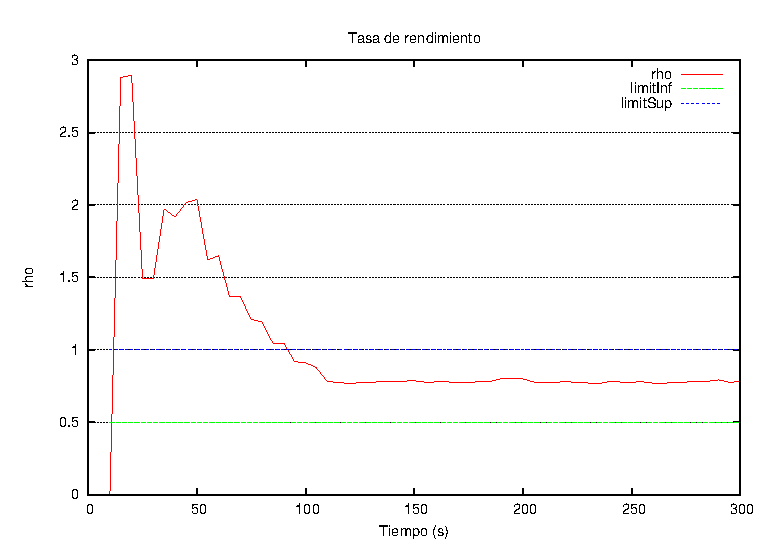
\includegraphics[scale=0.8]{images/Umbrales.eps}
  \caption{Comportamiento de la tasa de procesamiento de un operador.}
  \label{fig:umbrales}
\end{figure}


\section{Algoritmo predictivo}
Para la confección del algoritmo predictivo se realizó un análisis según las cadenas de Markov \citep{ching2006markov}, por lo que se tuvieron que seguir las siguientes etapas:

\begin{itemize}
	%\item Definir tiempo discretos, los cuales fueran cambiando con el tiempo según un proceso estocástico. Para esto se consideró el cambio del estado del sistema de período a otro, es decir, las transiciones existentes entre cada uno de los estados, ya sea ocioso, estable o inestable, en período de un segundo.
	\item Definir muestras en tiempos discretos, las cuales cambian con el tiempo según un proceso estocástico. Las muestras se definieron como la tasa de procesamiento ($\lambda$) del operador, la cual dependiendo del valor que poseyera, iba a otorgar un estado al operador.
	\item Determinar los estados finitos que se van a utilizar para la conformación de la cadena, que en este caso son los estados que se puede encontrar el operador: ocioso, estable o inestable.
	\item Una cantidad representativa de muestras para la construcción de la cadena de Markov en el período analizado. Estas muestras son independientes de un período y otro, por lo que los valores de la cadena de Markov irán cambiando en cada período de tiempo. Para la implementación del algoritmo, se consideraron cien muestras por cada período, cuyos intervalos son de cien segundos, valor establecido en base al trabajo de \citep{GongGW10}.
\end{itemize}

%Dato esto, se presentó un cadena de Markov en base a estas bases, como se refleja en la Figura \ref{fig:cadenaMarkovPredictiva}, donde existen tres estados, los cuales pueden ser ocioso, estable o inestable, y poseen ciertas transiciones de un estado a otro, cuyas probabilidades van a estar determinadas por la historia existente en el sistema.

%Dado esto, se construyó una cadena de Markov en base a la transición de un estado a otro del operador según la tasa de rendimiento, donde los tres posibles estados son ocioso, estable o inestable, donde exista una probabilidad de transición entre un estado a otro, cuyos valores estarán determinados por el historial del período analizado.

Tomando las bases anteriores, se diseño una cadena de Markov en base a tres posibles estados: ocioso, estable e inestable, como se demuestra en la Figura \ref{fig:cadenaMarkovPredictiva}. Cada uno de los estados posee una probabilidad de transición hacia algún estado, cuyas probabilidades están definidas por las muestras obtenidas en el período de tiempo analizado.

\begin{figure}[ht!]
  \centering
    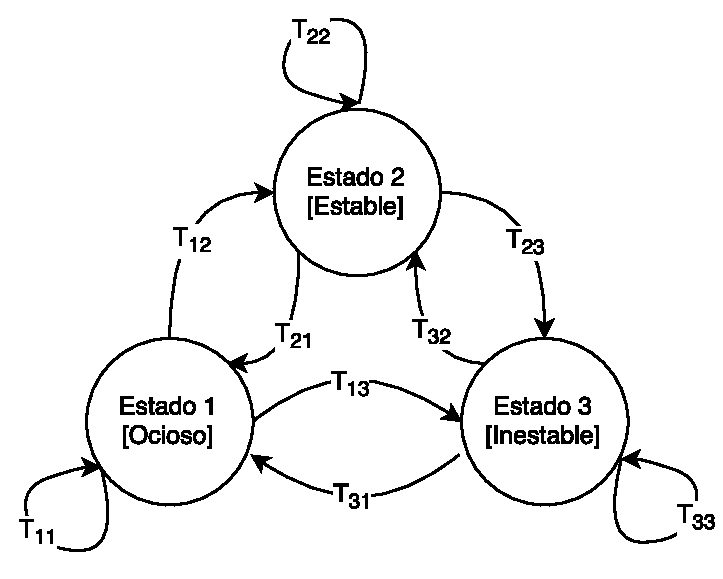
\includegraphics[scale=0.75]{images/CadenaMarkovPredictiva.pdf}
  \caption{Cadena de Markov dado el modelo propuesto del sistema.}
  \label{fig:cadenaMarkovPredictiva}
\end{figure}

%Por lo tanto, para cada operador existe una cadena de Markov según la historia existente en una ventana de tiempo. Para la generación de esta cadena de Markov, se puede ver en el Apéndice \ref{apendice:matrizTransicion} el algoritmo que crea la matriz de transición según el historial del operador, la cual corresponde a la tasa de rendimiento recolectada cada un segundo en la última ventana de tiempo del operador analizado. En la Ecuación \ref{eq:matrizTransicionPredictive} se puede ver la matriz de transición que se obtiene de la cadena de Markov de la Figura \ref{fig:cadenaMarkovPredictiva}, la cual posee una probabilidad de transición desde cada uno de los estado a otro existente.

Por lo tanto, para cada operador se construirá una cadena de Markov según el historial obtenido en la ventana de tiempo. Para la conformación de la cadena de Markov se consideraron las muestras de la historia, por lo que la transición de una muestra a otra presentaba un transición, las cuales dieron origen a la matriz de transición. En el Anexo \ref{apendice:matrizTransicion} se presenta el algoritmo que se empleó para construir la matriz de transición. En la ecuación \ref{eq:matrizTransicionPredictive} se muestra la matriz de transición que se obtiene de la cadena de Markov de la Figura \ref{fig:cadenaMarkovPredictiva}.

\begin{equation} \label{eq:matrizTransicionPredictive}
	P =
	\begin{bmatrix}
		T_{1,1} & T_{1,2} & T_{1,3} \\
		T_{2,1} & T_{2,2} & T_{2,3} \\
		T_{3,1} & T_{3,2} & T_{3,3}
	\end{bmatrix}	
\end{equation}

%Teniendo la matriz de transición de la cadena de Markov de un operador, se puede calcular la distribución estacionaria, la cual indica la probabilidad que a largo plazo se encuentre el sistema en cierto estado, ya sea ocioso, estable o inestable. Para el cálculo de esta, se utiliza la ecuación de Chapman-Kolmogórov \citep{Papoulis1984} expuesta en la subsección \ref{subsec:cadenaMarkov}.
Obtenida la matriz de transición se puede calcular la distribución estacionaria de la cadena de Markov, la cual indica las probabilidades que en el futuro se encuentra el operador esté en cada uno de los posibles estados, ya sea ocioso, estable o inestable. Para el cálculo de esto, se utiliza la ecuación de Chapman-Kolmogórov \citep{Papoulis1984} descrita en la subsección \ref{subsec:cadenaMarkov}.

El Algoritmo \ref{alg:distEstacionaria} describe el cálculo de la distribución estacionaria, cuya entrada es la matriz de transición de un operador del SPS. 

Antes de realizar el cálculo, es importante analizar si efectivamente existen transiciones en todos los estados, debido a que existía la posibilidad que no hubiera alguna transición a un estado en particular en un período de tiempo dado. Por ejemplo, puede ocurrir que en una ventana de tiempo nunca se ha alcanzado el estado ocioso en el sistema, pero si el estable o inestable. Como el cálculo de la distribución estacionaria requiere un estado de inicio, se verificó si efectivamente existía o no el estado, y en caso no existir, el estado de inicio será alguno existente.

%Al realizar las iteraciones correspondientes al cálculo, se proporcionó como entrada la cantidad que se estimaba necesario. Es importante destacar que entre mayor cantidad de iteraciones, mayor precisión existe en el cálculo, pero mayor es el tiempo de espera.
La cantidad de iteraciones que debe realizarse para el cálculo correspondiente, se proporcionó como parámetro entrada del algoritmo. Es importante destacar que entre mayor cantidad de iteraciones, mayor precisión en el valor de la predicción, pero esto implica a su vez un mayor tiempo de cómputo. Debido a esto, es que se trató de considerar un punto medio, de tal manera de tener un bajo margen de error, pero con bajo costo en el tiempo de ejecución. La cantidad de iteraciones escogida para la implementación fue de 100.000.

\begin{algorithm}[!ht]
	\caption{Cálculo de la distribución estacionaria de la cadena de Markov de un operador $\phi$.}
	\label{alg:distEstacionaria}
	\begin{algorithmic}[1]
	\REQUIRE $\Gamma$ Matriz de transición del operador $\phi$, $\upsilon$ cantidad de iteraciones deseadas y última muestra $m$ de las muestras de $\rho$
	\ENSURE $\Delta$ Distribución estacionaria de la cadena de Markov del operador $\phi$.
	\STATE $i \leftarrow 0$ \COMMENT {Estado inicial de iteración}
	\IF {$\rho_m < 0.5$}
		\STATE {$i \leftarrow 0$}
	\ELSIF {$0.5 \leqslant \rho_m \leqslant 0.5$}
		\STATE {$i \leftarrow 1$}
	\ELSE
		\STATE {$i \leftarrow 2$}
	\ENDIF
	
	\STATE $\tau \leftarrow Arreglo[3]$ \COMMENT {Contador para la normalizaci\'on de los datos}
	\FOR {$k=0$ a $\upsilon$}
		\STATE $u = randomUniform(0,1)$
		\STATE $\sigma = 0$
		\FOR {$j=0$ a $3$}
			\STATE $\sigma = \sigma + \Gamma_{i,j}$
			\IF {$u \leqslant  \sigma$}
				\STATE $\tau_{j}++$
				\STATE $i \leftarrow j$
				\STATE \textbf{break}
			\ENDIF
		\ENDFOR
	\ENDFOR

	\STATE $\Delta \leftarrow Arreglo[3]$ \COMMENT {Distribución estacionaria de la cadena de Markov del operador $\phi$}
	\FOR{$k=0$ a $3$}
		\STATE $\Delta_{k} \leftarrow \nicefrac{\tau_{k}}{\upsilon}$
	\ENDFOR	
	
	\RETURN $\Delta$
	
	\end{algorithmic}
\end{algorithm}

Obtenida la distribución estacionaria, se procede a analizar las probabilidades obtenidas y como influye al operador. Para esto, se consideró que las probabilidades tuvieron entre ellas una desviación estándar superior a 0.25, debido que si esto se cumple, la probabilidad mayor de la distribución estacionaria no posee incertidumbre \citep{soong2004fundamentals}, porque en caso que no supere la desviación estándar, puede ser que dos probabilidades sean muy parecidas y la probabilidad no sea un comportamiento determinante. En el Algoritmo \ref{alg:predictive} se describe el análisis que se realiza a la distribución estacionaria, siendo en primer lugar el análisis estadístico de las probabilidades, y segundo la obtención del estado con mayor valor de las probabilidades, retornando finalmente el estado del operador. Cabe destacar que el primer estado se consideró ocioso, el segundo estable, y el tercero inestable.

\begin{algorithm}[!ht]
	\caption{Algoritmo predictivo del sistema de distribución de carga.}
	\label{alg:predictive}
	\begin{algorithmic}[1]
	\REQUIRE$\Delta$ Distribución estacionaria de la cadena de Markov del operador $\phi$.
	\ENSURE Estado a futuro del operador, donde -1 significa estado ocioso, 0 estable y 1 inestable.
	\IF {$\sigma(\Delta_1,\Delta_2,\Delta_3) > 0.25$ \COMMENT {Desviaci\'on est\'andar de las probabilidades de la distribuci\'on estacionaria}} 
		\STATE $i \leftarrow getStateMax(\Delta)$ \COMMENT {Obtención del estado con mayor probabilidad}
		\IF {$i=1$}
			\RETURN -1
		\ELSIF {$i=2$}
			\RETURN 0			
		\ELSE
			\RETURN 1
		\ENDIF
	\ENDIF
	
	\RETURN 0
	
	\end{algorithmic}
\end{algorithm}

\section{Administración del sistema}

El último componente del sistema es el administrador de réplicas, cuya función es administrar la cantidad de réplicas en cada uno de los operadores según los recursos disponibles por parte del sistema y según el estado que adopte un operador, ya sea a futuro o en el momento.

%Para esto, se diseño un administrador que se ejecutara según el período que se encuentra el algoritmo reactivo o predictivo, donde cada período es de 19 ejecuciones del algoritmo reactivo y 1 del algoritmo reactivo. Esto fue pensando dado que cada cien segundos se poseían las muestras suficientes para el análisis del algoritmo predictivo, por lo tanto, cada ejecución del algoritmo reactivo iba a ser cada cinco segundos, de esa manera al segundo cien iba a realizarse en vez del algoritmo reactivo, el predictivo ya que posee la cantidad suficiente de muestras para su análisis.
Para esto, se diseño un administrador que ejecuta un algoritmo (reactivo o predictivo) según el período del ciclo que se encuentre el sistema. Cada ciclo posee 20 períodos, donde los primeros 19 corresponde al algoritmo reactivo y el último corresponde al algoritmo predictivo. Cada período posee un intervalo de 5 segundos, de esta manera, cada ciclo tendrá un intervalo de 100 segundos, la cantidad necesaria para obtener las muestras para el algoritmo reactivo, suponiendo que cada muestra es obtenida en 1 segundo.

\begin{algorithm}[!ht]
	\caption{Administración de réplicas de un operador $\phi$ dado su comportamiento en el sistema de distribución de carga.}
	\label{alg:administracion}
	\begin{algorithmic}[1]
	\REQUIRE Operador $\phi$ a analizar y $\iota$ período en que se encuentra el sistema de distribución de carga.
	\ENSURE Cantidad de réplicas a modificar del operador.	
	
	\IF {$\iota \mod{20} \neq 0 $}
		\STATE $\delta_{\iota} \leftarrow AlgoritmoReactivo(\phi)$
		\IF {$\delta_{\iota}$ \AND $\delta_{\iota-1}$ son estado inestable}
			\IF {No excede la cantidad máxima de réplicas en el sistema}
				\STATE $\delta_{\iota} \leftarrow \text{estado estable}$ 
				\RETURN Crear una réplica del operador $\phi$
			\ENDIF
		\ELSIF {$\delta_{\iota}$ \AND $\delta_{\iota-1}$ son estado ocioso}
			\RETURN Remover una réplica del operador $\phi$
		\ENDIF 
	\ELSE
		\STATE $\delta_{\iota} \leftarrow AlgoritmoPredictivo(\phi)$
		\IF {$\delta_{\iota}$ es estado inestable}
			\IF {No excede la cantidad máxima de réplicas en el sistema}
				\RETURN Crear cinco réplicas del operador $\phi$
			\ENDIF
		\ELSIF {$\delta_{\iota}$ es estado ocioso}
			\RETURN Remover cinco réplicas del operador $\phi$
		\ENDIF
	\ENDIF
	
	\RETURN No hacer nada al operador $\phi$
	
	\end{algorithmic}
\end{algorithm}

En el Algoritmo \ref{alg:administracion} está el procedimiento de administración, donde primero analiza que tipo de algoritmo debe ejecutar según el período del ciclo. En caso de realizarse el reactivo, se analiza si existen dos alertas consecutivas del mismo estado del operador, ya sea ocioso o inestable, y de ser así, realizar una modificación a la cantidad de réplicas del operador. Además, se cambió el estado del operador a estable, de tal manera de no considerar ese período para el próximo análisis reactivo, esto se consideró para dejar un margen de descanso para el algoritmo reactivo. Por otra parte, de ejecutarse el módulo predictivo, se analiza cual fue la predicción, por lo que si es ocioso disminuirá la cantidad de réplicas y si es inestable las aumentará. Como el proceso de predicción se realiza con menor frecuencia y posee mayor cantidad de cómputo, se considero que debía crear o remover mayor cantidad de réplicas que en el módulo reactivo, aprovechando así el análisis de la historia del operador.

Dentro de las consideraciones que se tuvieron para el diseño del administrador, fue la cantidad máxima de réplicas que podían realizarse. Dado que una de las limitantes de este trabajo fue que sólo se utilizó una máquina, la cantidad de recursos son limitados, por lo que aumentar la cantidad de réplicas indefinidamente iba a generar una sobrecarga en los recursos disponibles por parte de la máquina.